\documentclass[11pt,a4paper]{article}

\usepackage{siunitx}
%\usepackage[version=4]{mhchem}
\usepackage{multirow}
\usepackage{subfig}

\usepackage{pgfgantt}
%\usepackage{pdflscape}
% \usepackage[a4paper,margin=1in,landscape]{geometry}

% \usepackage[pdftex]{color,graphicx}
% \pagestyle{plain}
\usepackage{geometry}
\usepackage{rotating}
\usepackage{hyperref}

\newcommand{\ts}{\textsuperscript}
\newcommand{\ic}{\texttt}
\newcommand\todo[1]{\textbf{TODO: #1}}

\sisetup{detect-weight=true, detect-family=true}

\usepackage[backend=biber,style=authoryear,sorting=nyt,dashed=false]{biblatex}
\renewcommand*{\nameyeardelim}{\addcomma\space}
\addbibresource{references/references.bib} % note the .bib is required

%Wrong spellings!
%parameterization (unless part of someone else's work)
%parameterizing
%Paracon

\begin{document}

% \newgeometry{margin=2.0cm}
\newgeometry{margin=2.2cm, top=2.5cm}

\begin{center}
    \Large{\textbf{Monitoring Committee Report V}}\\[0.1cm]
    \large{Mark Muetzelfeldt}\\
    \normalsize{11am on Thursday 14\ts{th} December 2017 in 2U13}\\[0.1cm]		
    \rule{\textwidth}{0.2mm}
    \textbf{Project Title: }Development of scale-awareness in the representation of
    convective cloud systems\\
    \textbf{Monitoring Committee: }Dr Omduth Coceal and  Dr Andrew Turner\\
    \textbf{Supervisors: }Prof. Robert Plant, Prof. Peter Clark, Dr Steve Woolnough \\
    and Dr Alison Stirling (Met Office CASE supervisor)\\
    \rule{\textwidth}{0.2mm}
\end{center}

\section{Project overview}
\label{sec:Project Overview}
% Where have I been, where am I and where am I going.

% Overall goal.
% * represent the org of convection in a conv p13n
% * do in a scale-aware way.
% Steps to do this (see thesis structure notes)
% Stress physically justifiable
% Point out links/deps between hi-res <=> p'trized
With Monitoring Committee V comes the extra requirement of detailed planning of the rest of my PhD. This is a useful exercise in its own right, and focuses my mind on the tasks of generating the results and writing up my thesis. It is also a good time to take stock and think about what I have done to date, how to bring this together into a coherent thesis and what gaps there might be in this thesis.

I started out getting up-to-speed with meteorology and numerical modelling, completing 6 assessed modules. This was followed by learning about the fields of convective parametrization and high-resolution modelling, putting into practice a lot of what I learnt by running the idealized UM (iUM). In phase 0 of my PhD plan, the goal was to make sure that the iUM was capable of being used for what we wanted to do; this has been done but took longer than expected due to the moisture conservation issues highlighted in previous MCs. Subsequent work, leading up to the companion paper for MC IV, built on learning how to use the iUM and on understanding and managing its flaws for high-resolution modelling. I also spent time reading up on the organization of convection, in the atmosphere in the form of squall lines, and in models in the form of squall lines, and through the mechanism of self-aggregation.

To indicate how I will turn this work into a thesis, it is useful to set out the logical line of argument of my thesis. The goal remains to represent shear-induced organization of convection in a convective parametrization scheme, ideally in a way that is scale-aware. The line of argument starts by recognizing that shear can have an organizing effect on cloud fields. By looking at the range of wind profiles generated in coarse-resolution models, I will build a number of Representative Wind Profiles (RWPs), that reduce the parameter space to something manageable. The second strand is to use high-resolution models to investigate how shear-induced organization affects key aspects of the cloud field, for example the lifetime of the convection, the vertical momentum transports and the statistics of mass flux in the cloud field. This information, coupled with a diagnosis of which RWP a given grid-column is in, can then be used to modify the convective parametrization scheme in the coarse-resolution model.

There are still blanks to be filled in in the remaining part of my PhD. How to generate the RWPs? I have done some experimental work to classify these profiles using a machine learning technique, but this needs to be extended and the analysis checked more thoroughly (see section XXX). How to modify the convective parametrization? We have some ideas how this could work (see section XXX), but these will need to be tested. 

Overall, I am pleased with how my PhD is going. Although I have not accomplished all the things laid out in last MC report's ``Future work'' section, I believe I have done an equivalent amount of work. My placement at the Met Office meant that it was sensible to re-arrange the order in which I carried out my PhD plan, looking into how I might go about modifying a convective parametrization scheme before carrying out some of the high-resolution modelling. Finding a potential way of reducing the parameter space of the shear profiles also means that the high-resolution modelling has been pushed further back in my updated plan. 

\subsection{Background reading}
\label{sec:Background reading}

% Conv p13n + org.
% Mapes and Neale 2011
% Willet and Whitall 2017
% Tompkins and Semie 2017
% Shear climatology
% Aiyyer and Thorncroft 2006
% Houchi et al. 2010
% Bonus
% Davies et al. 2009

To start to get to grips with some work looking at wind profile and shear climatologies, I read \cite{houchi2010comparison}. They look into the zonal and meridional profiles of $u$ and $\frac{du}{dz}$ in both radiosonde observations and ECMWF \SI{12}{hr} forecasts. Although the motivation of the work is different from mine, they are interested in using the ECMWF forecasts to model how a satellite will perform, some of the ideas may be useful and it is something to compare against. However, they were looking at comparisons between co-located observations and interpolated model output, and they were interested in a larger depth of atmosphere, from the surface to \SI{35}{km}.

In \cite{mapes2011parameterizing}, they look at the link between entrainment as formulated in a convective parametrization and the behaviour of the model. They identify the ``entrainment dilemma'', whereby a value of the entrainment rate that is too high leads to a model that is unstable to explicit convection. Conversely, an entrainment rate that is too low leads to too much deep convection, and a corresponding deterioration of the space and time distributions and variability. To ameliorate this situation, the develop a 2D dimensionless prognostic \textit{org} that represents then subgrid organization of a given grid-column. Rain evaporation is taken as a source or \textit{org}, which can be advected horizontally. \textit{org} acts to reduce the entrainment rate in a grid-column, thereby acting as a time-lagged positive feedback on the parametrized convection. 

\cite{willett2017simple} take a similar approach. They again change the entrainment rate through a new prognostic variable. This time it is a 3D prognostic variable, which they argue makes it simpler to advect around as there is not need to work out an effective steering level as in \cite{mapes2011parameterizing}. The source of the prognostic is taken as being the precipitation, as this is related to the strength of the convection.

Finally, a look at \cite{tompkins2017organization} examines entrainment affects organization from a different perspective - that of a Cloud Resolving Model (CRM). In my project, I am aiming to link entrainment in the convective parametrization to results from a CRM, so this serves as an introduction to some of the concepts involved. ...

\section{Completed work}
\label{sec:Completed work}

\subsection{Progress overview}
\label{sec:Progress overview}

In terms of sticking to the work laid out in the last MC, I have made good progress on cloud tracking, doing all the work presented here at \SI{1}{km} resolution (Section \ref{sec:Cloud tracking}). I worked on reducing the spin-up time by using lower-resolution profiles of $\theta$ and water vapour, work which will be even more useful in terms of saving computation time at higher resolution. I have not done more work at \SI{250}{m} resolution yet, nor have I run a stochastic parametrization scheme in either idealized or global simulations. Instead, I laid the foundations for other parts of my PhD with the shear classification work and making modifications to the \cite{gregory1990mass} scheme as set out in Sections \ref{sec:Classification of shear profiles} and \ref{sec:um_mod}.

\subsection{Cloud tracking}
\label{sec:Cloud tracking}

%\cite{wilson1998nowcasting},  \cite{plant2009statistical}

From analysing cloud tracks, useful information can be gleaned on e.g. cloud lifetimes that I might be able to use to modify a convective parametrization scheme. The cloud tracking used here uses an approach that is a combination of Juwon Kim's cloud tracking and the method of \cite{plant2009statistical}. 
%The reason that I chose not to use Juwon's work without modification was that it was developed for a different reason - tracking clouds in real world situations with a changing wind vector across the domain (my idealized work used a constant wind over the domain). \cite{plant2009statistical} method was integrated directly into the model, this was not possible for me although the bulk of the ideas come from this method. 
The method works by comparing two snapshots of the cloud field at a given height a certain time apart, in my case I use \SI{2}{km} and \SI{5}{min}. To calculate overlaps, the maximum correlation vector between the two fields is calculated, and this is used to project the cloud field at the first snapshot to where it would be moved to by the time of the second snapshot. This idea and code was taken from Juwon's method. Then the method of \cite{plant2009statistical} is applied, working out the number of merges and splits and handling edge cases such as when two clouds split and merge into two separate clouds (see Figure \todo{XXX}).

I then applied this method to data from the last \todo{XXX} days from a \SI{1}{km} resolution run, the results from the no shear and strong shear experiments (S0 and S4) are presented in Figure \ref{fig:cloud_lifetimes}. 
The distribution is bimodal, with the first mode showing a large number of short-lived clouds. The second mode peaks at a lifetime of around \SI{50}{min}. 
The results from S0 for all cloud lifetimes are in line with previous modelling work \cite{plant2008stochastic} and observations \todo{cite}.

The distribution can be further analysed by splitting it into simple and complex lifetimes - lifetimes that contain no merges or splits and those that do. The complex lifetimes distribution for S0 is shown in subfigure \ref{fig:cloud_lifetimes} (b), where it is seen that complex lifetimes are longer than all lifetimes, and there are far fewer with very short lifetimes. 

Comparing the equivalent subfigures for S4, two main points jump out. The first is that the number of short-lived clouds for all lifetimes is increased. Speculatively, this could be due to enhanced shear above the boundary layer increasing entrainment and therefore decreasing cloud lifetime. The second is that for S4, the distribution is shifted towards longer lifetimes. The mean lifetime for these clouds is \todo{XXX}, whereas for S0 it is \todo{XXX}.

\begin{figure}[htp!]%
    \centering
    \subfloat[S0, all lifetimes]{{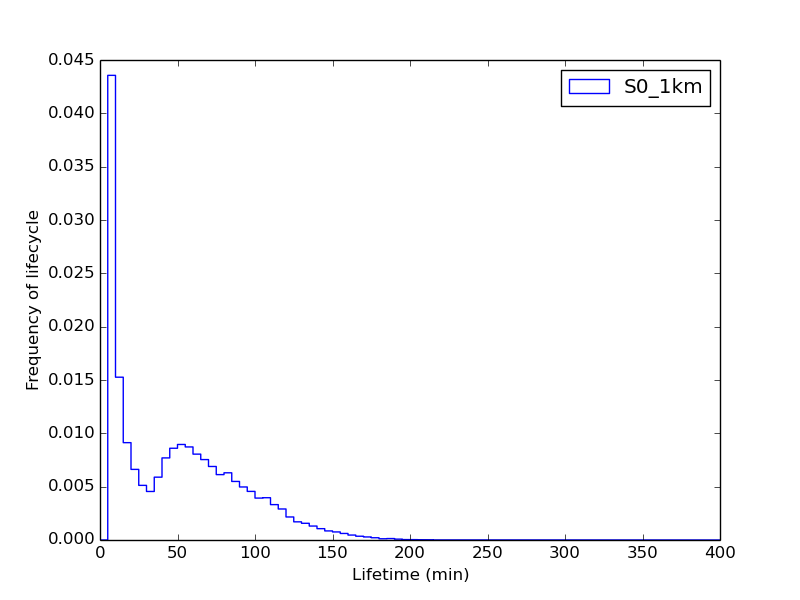
\includegraphics[width=7cm]{figs/atmos_S0_1km_cloud_tracking_z1_t1_all_lifetimes.png} }}%
    \qquad
    \subfloat[S0, complex lifetimes]{{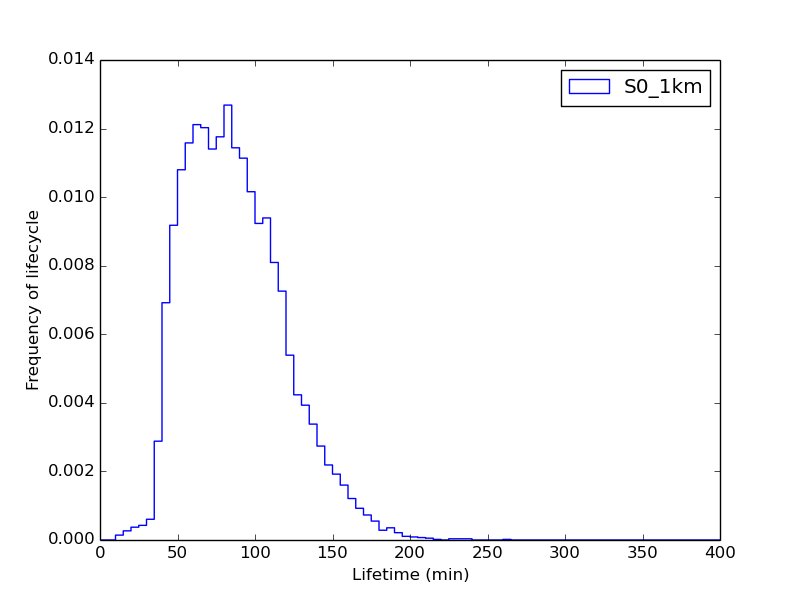
\includegraphics[width=7cm]{figs/atmos_S0_1km_cloud_tracking_z1_t1_nonlinear_lifetimes.png} }}%
    \qquad
    \subfloat[S4, all lifetimes]{{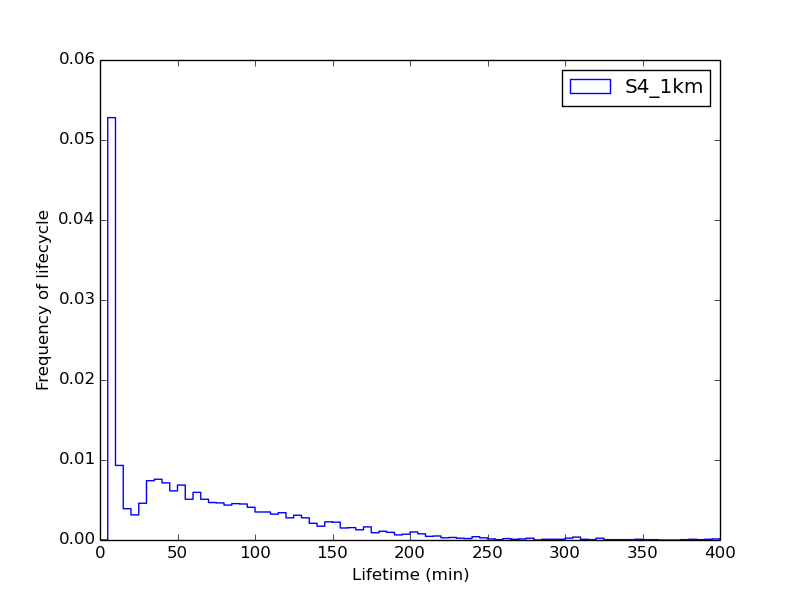
\includegraphics[width=7cm]{figs/atmos_S4_1km_cloud_tracking_z1_t1_all_lifetimes.png} }}%
    \qquad
    \subfloat[S4, complex lifetimes]{{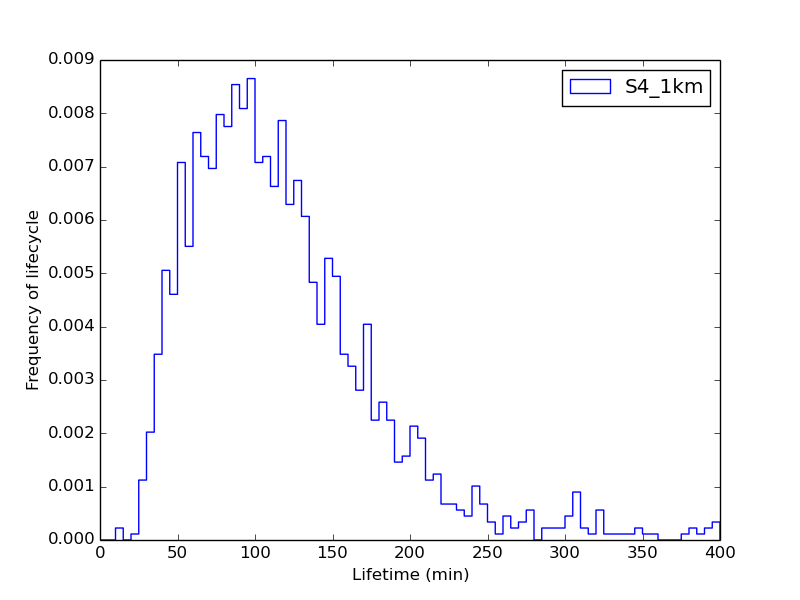
\includegraphics[width=7cm]{figs/atmos_S4_1km_cloud_tracking_z1_t1_nonlinear_lifetimes.png} }}%
    \caption{Distribution of cloud lifetimes for S0 (top) and S4 (bottom). Left shows all cloud lifetimes, right shows complex lifetimes only. Statistics were gathered over 10 days of simulation.}%
    \label{fig:cloud_lifetimes}%
\end{figure}

\subsection{Classification of shear profiles}
\label{sec:Classification of shear profiles}

My work so far has been oriented towards understanding how shear affects cloud fields. However, the aim is to information from this work to modify a convective parametrization scheme. This requires being able to link the shear as seen by a model grid-column, to some change to the parametrization scheme. One way of doing this is to classify the shear in a grid-column, as presented here.

To find the shear profiles for classification, I ran a standard Met Office GA7.0 run (vn10.7 \todo{check}). Initially, I ran this for one day, and took results from the tropics (defined as \ang{30}N - \ang{30}S) at a frequency of every \SI{6}{hr}. I outputed the $u$ and $v$ profiles on 6 pressure levels of: \SI{900}, \todo{get}, \SI{200}{hPa}. The profiles were optionally filtered based on whether there was CAPE $>$ \SI{500}{J.kg^{-1}} or grid-scale ascent (w $>$ \SI{0}{m.s^{-1}}. To group the profiles, I turned each pair of $u$ and $v$ profiles into one sample with 12 values or dimensions, and ran a Principal Component Analysis algorithm on it to reduce the number of dimensions to 5 (this explains over 90\% of the variance of the profiles). I then ran a k-means clustering algorithm to group the profiles.

Figure \ref{fig:shear_profiles} shows the results from this analysis, with the profiles being filtered on CAPE $>$ \SI{500}{J.kg^{-1}}. Subfigure (a) shows a reasonably successful grouping, the low level shear is aligned for both wind components and the spread between the profiles is not too large. Subfigure (b) shows a group of profiles where the process has been less successful; there is large spread between the different profiles at all levels and important features in some profiles are not seen in others.

This is a work in progress. I would like to continue this over the next couple of months because I believe it holds promise for linking the two strands of my thesis. My supervisors and I have discussed ways in which this could be improved, such as deciding which of these profiles are interesting from a shear perspective, processing the profiles first to normalize them about a given shear angle and removing the dependence on higher levels as this is unlikely to affect shear induced organization.

\begin{figure}[htp!]%
    \centering
    \subfloat[]{{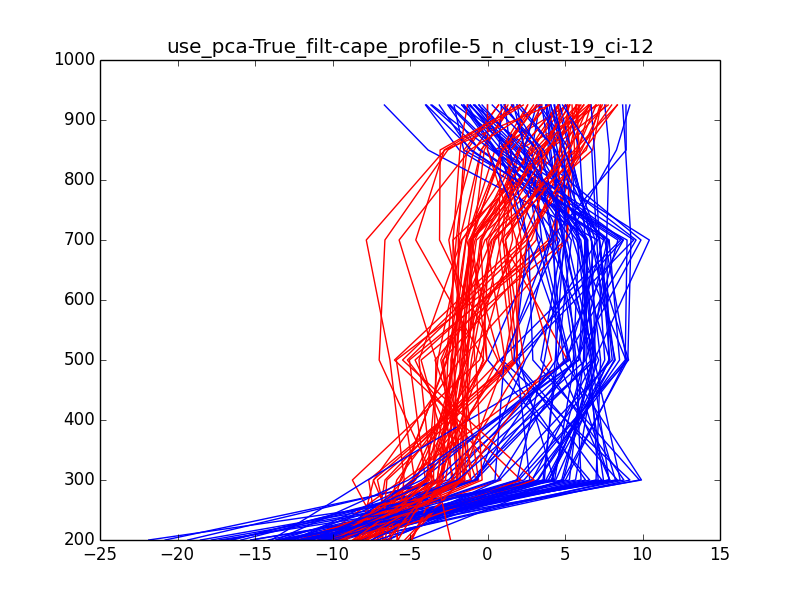
\includegraphics[width=7cm]{figs/atmos_None_shear_profile_classification_analysis_use_pca-True_filt-cape_profile-5_n_clust-19_ci-12.png} }}%
    \qquad
    \subfloat[]{{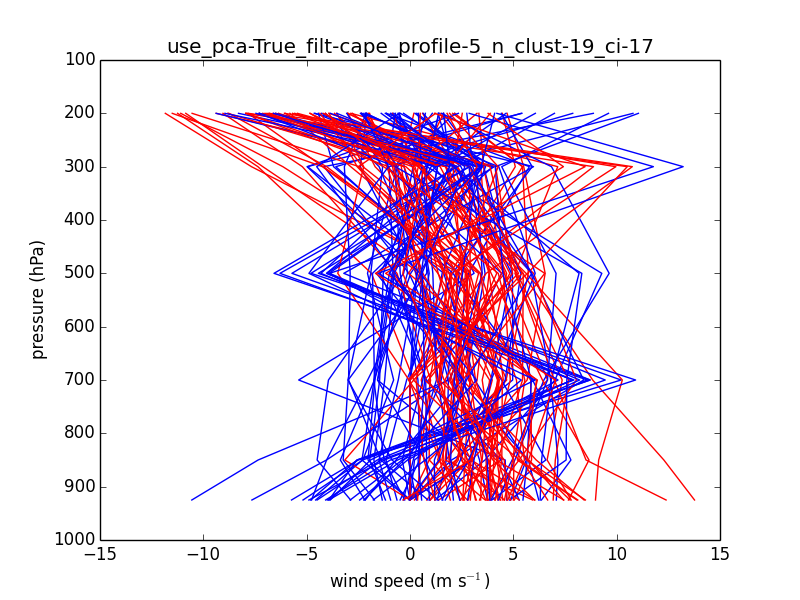
\includegraphics[width=7cm]{figs/atmos_None_shear_profile_classification_analysis_use_pca-True_filt-cape_profile-5_n_clust-19_ci-17.png} }}%
    \caption{\todo{invert y-axis!} Shear profiles classified into different RWPs, $u$ is blue and $v$ is red. (a) shows reasonable classification success with relatively distinct profiles classified together, whereas (b) shows large variation between the individual profiles.}%
    \label{fig:shear_profiles}%
\end{figure}


\subsection{Modifications to the UM based on shear}
\label{sec:um_mod}

When I was on my Met Office placement (see Section \ref{sec:Met Office placement}), I learnt how to make modifications to the UM. The goal was to add a link between the shear in a grid-column to the convection scheme. The emphasis at this stage was more in terms of the technicalities of how to make the changes rather than exactly what changes to make, although the final changes I make may well end up being similar to what I have done. The change was to modify the entrainment rate of the scheme based on the shear in a grid-column, taking a cue from my work looking at cloud lifetimes in CRMs. The difficulty is that the work I have done on lifetimes suggests that I should change something corresponding to the cumulus lifetime in the parametrization scheme, however \cite{gregory1990mass} has no such parameter. Therefore shear was chosen as an expedient proxy to this for now. N.B. other schemes, such as \cite{plant2008stochastic} do represent this explicitly, and therefore might be more suitable 

The modifications involved adding in new diagnositcs: the bulk shear and the Bulk Richardson Number (BRN). They also involved passing namelist settings into the UM to e.g. turn the new `shear aware' scheme on. The shear information had to be passed into the convection scheme to where the entrainment rate is calculated, and used to modify this. Given that my knowledge of Fortran had been fairly superficial before now, I also had to learn about some of its quirks. I made changes in keeping with the Met Office's best practices, creating a ticket (#3599) and branch to describe and implement that changes.

To verify the new diagnostics I had added were correct, I outputted some standard ($\theta$, $u$, $v$, orography) to perform the same calculation offline in Python. This involved careful matching up of horizontal C-grids, Charney-Phillips staggered vertical grids and $\sigma$ scaled height coords as well as outputting the standard data one timestep before the new diagnostic. After numerous bugs, mainly due to array indexing/passing into subroutines, had been found and eliminated, good agreement was seen between the two calculations (differences were small and I believe due to the packing precision of the diagnostics).

From here I could use the BRN to affect the deep convection scheme. The change was rather arbitrary - a BRN $<$ 10 was used to reduce the entrainment by 5\%. Examined over the course of 1 day, the change had a small but growing effect on the model state, indicating that the code was being exercised and was having an effect. I will be able to build on this work when it comes to running the parametrized tests later in my PhD.

\section{Future work}
\label{sec:Future work}

\subsection{Shear climatology in the UM}
\label{sec:Shear climatology in the UM}

\subsection{High-resolution idealized modelling}
\label{sec:High-resolution idealized modelling}

\subsection{Writing 1}
\label{sec:Writing 1}

\section{Training record}
\label{sec:Training record}
% CMSS
% RRDPs

\subsection{Met Office placement}
\label{sec:Met Office placement}

\subsection{Posters, presentations and conferences}
\label{sec:presentations}
% Cambridge plenary
% Delft

\subsection{Transferable skills}
\label{sec:Transferable skills}
% PGR forum co-chair + org of QV.

\printbibliography[title={References}]

\newpage
\section*{Appendix}

\subsection*{PhD Timetable}

\begin{ganttchart}[vgrid, hgrid, y unit chart=0.75cm, MC/.style={milestone/.append style={shape=circle}}]{1}{20}  % <---
    \gantttitle{2017}{2}
    \gantttitle{2018}{12}
    \gantttitle{2019}{6} \\
    \gantttitle{N}{1}
    \gantttitle{D}{1}
    \gantttitle{J}{1}
    \gantttitle{F}{1}
    \gantttitle{M}{1}
    \gantttitle{A}{1}
    \gantttitle{M}{1}
    \gantttitle{J}{1}
    \gantttitle{J}{1}
    \gantttitle{A}{1}
    \gantttitle{S}{1}
    \gantttitle{O}{1}
    \gantttitle{N}{1}
    \gantttitle{D}{1}
    \gantttitle{J}{1}
    \gantttitle{F}{1}
    \gantttitle{M}{1}
    \gantttitle{A}{1}
    \gantttitle{M}{1}
    \gantttitle{J}{1} \\
    \ganttmilestone[MC, milestone left shift=0.2,milestone right shift=-0.2]{Monitoring committees}{2} 
    \ganttmilestone[MC, milestone left shift=0.2,milestone right shift=-0.2]{}{8} 
    \ganttmilestone[MC, milestone left shift=0.2,milestone right shift=-0.2]{}{14}  \\
    \ganttbar{Shear climatology}{2}{3} \\
    \ganttbar{High-resolution modelling}{3}{5} 
    \ganttmilestone{}{5} \\
    \ganttbar{Writing 1}{6}{8} 
    \ganttmilestone{}{8} \\
    \ganttbar{Idealized parametrized}{9}{11} \\
    \ganttbar{Global parametrized}{11}{13} 
    \ganttmilestone{}{13} \\
    \ganttbar{Writing 2}{13}{17} 
    \ganttmilestone{}{17} 
\end{ganttchart}

\subsection*{Repositories}

\begin{itemize}
  \item managing UM output: \href{https://github.com/markmuetz/omnium}{omnium}
  \item high-resolution analysis: \href{https://github.com/markmuetz/scaffold_analysis}{scaffold\_analysis}
  \item climatology of shear analysis: \href{https://github.com/markmuetz/cosar_analysis}{cosar\_analysis}
\end{itemize}

% Around 400 words.
\subsection*{Training record}
\subsubsection*{Year 1}

\begin{itemize}
  \item RRDP: Intermediate/Advanced \LaTeX\ (4/11/2015)
  \item RRDP: You and your supervisor (11/11/2015)
  \item RRDP: Quality assurance in research (18/11/2015)
  \item RRDP (equivalent): UM Training (16-18/12/2015)
  \item RRDP (equivalent): Preparing to teach: Introduction to teaching and learning (26/1/2016)
  \item Preparing to teach: Marking and feedback (26/1/2016)
  \item Preparing to teach: Laboratory demonstrating and leading small groups (27/1/2016)
  \item MONC Training course (9-10/2/2016)
  \item RRDP (equivalent): Fairbrother Lecture ``A slippery situation: melting ice in Antarctica'' (4/5/2016)
  \item ECMWF Parametrization of subgrid physical processes (16-20/5/2016)
\end{itemize}

\subsubsection*{Year 2}

\begin{itemize}
  \item RRDP: Managing your research project (17/11/2016)
  \item RRDP: How to write a thesis (24/1/2017)
  \item SCENARIO Data Assimilation Course (14-15/2/2017)
  \item RRDP: Presentation skills (7/3/2017)
  \item Software Development for scientists (8/3/2017, 28-29/3/2017)
\end{itemize}

\subsubsection*{Year 3}

\begin{itemize}
  \item NCAS Climate Modelling Summer School: demonstrating Numerical Methods for Hilary Weller (11-15/11/2017)
  \item CASE Met Office Placement (30/10/2017 - 24/11/2017)
  \item RRDP: Open access for research publications (27/11/2017)
  \item RRDP: Introduction to impact (30/11/2017)
\end{itemize}

\subsection*{Talks and conferences attended}

\begin{itemize}
  \item Climate Change 2013: The physical science basis. Institute of Physics (2/2014)
  \item Dame Julia Slingo: Taking the planet into uncharted territory: What climate models can tell us about the future (9/2014)
  \item SCENARIO NERC DTP Conference (9/6/2015)
  \item Climate Change in the run-up to the Paris conference: what has Physics got to say? (6/11/2015)
  \item RMetS talk: The risk and vulnerability of Europe to severe convective storms (6/4/2016)
  \item ParaCon Plenary 1 in Reading (27-28/6/2016)
  \item RMetS debate: What will make the public and politicians take climate change more seriously? (5/10/2016)
  \item RMetS talks: Come Rain or Come Shine (19/10/2016)
  \item COP22 Marrakech: Remote participation (11/11/2016)
  \item ParaCon plenary 2 in Leeds (6-7/12/2016)
  \item RMetS talks: Chaos and Confidence in Weather Forecasting (14/12/2016)
  \item ParaCon plenary 3 in Cambridge (3-4/7/2017)
  \item The Future of Cumulus Parametrization, Delft University of Technology (10-14/7/2017)
  \item ParaCon plenary 4 in Exeter (18-19/12/2017)
  \item (Planned) EGU: Vienna (8-13/4/2018)
\end{itemize}

\subsection*{Talks and conferences presented at}

\begin{itemize}
  \item Presentation: ``Effects of Shear on Cloud Field Organization''. \textit{Quo Vadis}, University of Reading (1/2/2017)
  \item Poster: ``Effects of Shear on Cloud Field Organization''. Met Office Academic Partnership (MOAP), Met Office, Exeter (22/2/2017)
  \item Poster: ``Effects of Vertical Shear on Cloud Field Organization and Variability''. The Future of Cumulus Parametrization, Delft University of Technology (10-14/7/2017)
  \item Poster: ``Effects of Vertical Shear on Cloud Field Organization and Variability''. PhD Poster Session (21/9/2017)
\end{itemize}

\end{document}
